\documentclass{article}
\usepackage[svgnames]{xcolor}
\usepackage[utf8]{inputenc}
\usepackage{pdfpages}
\usepackage{float}
\usepackage{fullpage} % Package to use full page
\usepackage{parskip} % Package to tweak paragraph skipping
\usepackage{tikz} % Package for drawing
\usepackage{amsmath}
\usepackage{hyperref}
\hypersetup{
    colorlinks=true,
    linkcolor=purple,
    filecolor=magenta,      
    urlcolor=pink,
}
\usepackage{amssymb}
\usepackage{bm}
\usepackage{framed}
\usepackage{amsthm}
\usepackage{listings}
\usepackage{biblatex}

\lstset{language=R,
    basicstyle=\small\ttfamily,
    stringstyle=\color{DarkGreen},
    otherkeywords={0,1,2,3,4,5,6,7,8,9},
    morekeywords={TRUE,FALSE},
    deletekeywords={data,frame,length,as,character},
    keywordstyle=\color{blue},
    commentstyle=\color{DarkGreen},
}

\addbibresource{glm-exercises.bib}

\newenvironment{lyxcode}
	{\par\begin{list}{}{
		\setlength{\rightmargin}{\leftmargin}
		\setlength{\listparindent}{0pt}% needed for AMS classes
		\raggedright
		\setlength{\itemsep}{0pt}
		\setlength{\parsep}{0pt}
		\normalfont\ttfamily}%
	 \item[]}
	{\end{list}}


\newcommand\independent{\protect\mathpalette{\protect\independenT}{\perp}}
\def\independenT#1#2{\mathrel{\rlap{$#1#2$}\mkern2mu{#1#2}}}

\newcommand{\E}{\mathrm{E}}
\newcommand{\Var}{\mathrm{Var}}
\newcommand{\Cov}{\mathrm{Cov}}
\newcommand{\Cor}{\mathrm{Cor}}

% vertical line in {bmatrix}
\makeatletter
\renewcommand*\env@matrix[1][*\c@MaxMatrixCols c]{%
 \hskip -\arraycolsep
 \let\@ifnextchar\new@ifnextchar
 \array{#1}}
\makeatother

\title{Exercises in Generalized Linear Models \\ \textbf{Week 46}}
\author{Vinnie Ko, Jonas Moss}
\date{Fall 2020}

\begin{document}
\maketitle
Exercises for the course \href{https://www.uio.no/studier/emner/matnat/math/STK3100/}{STK3100/STK4100: Introduction to Generalized Linear Models} at the University of Oslo, fall 2020. The exercises are from the textbook Alan Agresti: \textit{Foundations of Linear and Generalized Linear Models}. Wiley, 2015. ISBN: 978-1-118-73003-4. The additional exercises are available \href{https://www.uio.no/studier/emner/matnat/math/STK3100/h20/oppgaver.html}{online}. Exercises exclusively nvolving \texttt{R} are not covered.
9.22, 9.24, 9.29, and 9.39
\input{book-exercises/exercise-9.22}
\input{book-exercises/exercise-9.24}
\input{book-exercises/exercise-9.29}
\input{book-exercises/exercise-9.39}
\includepdf[pages = {2, 3, 4}]{exam-exercises/exam-2013-solution.pdf}
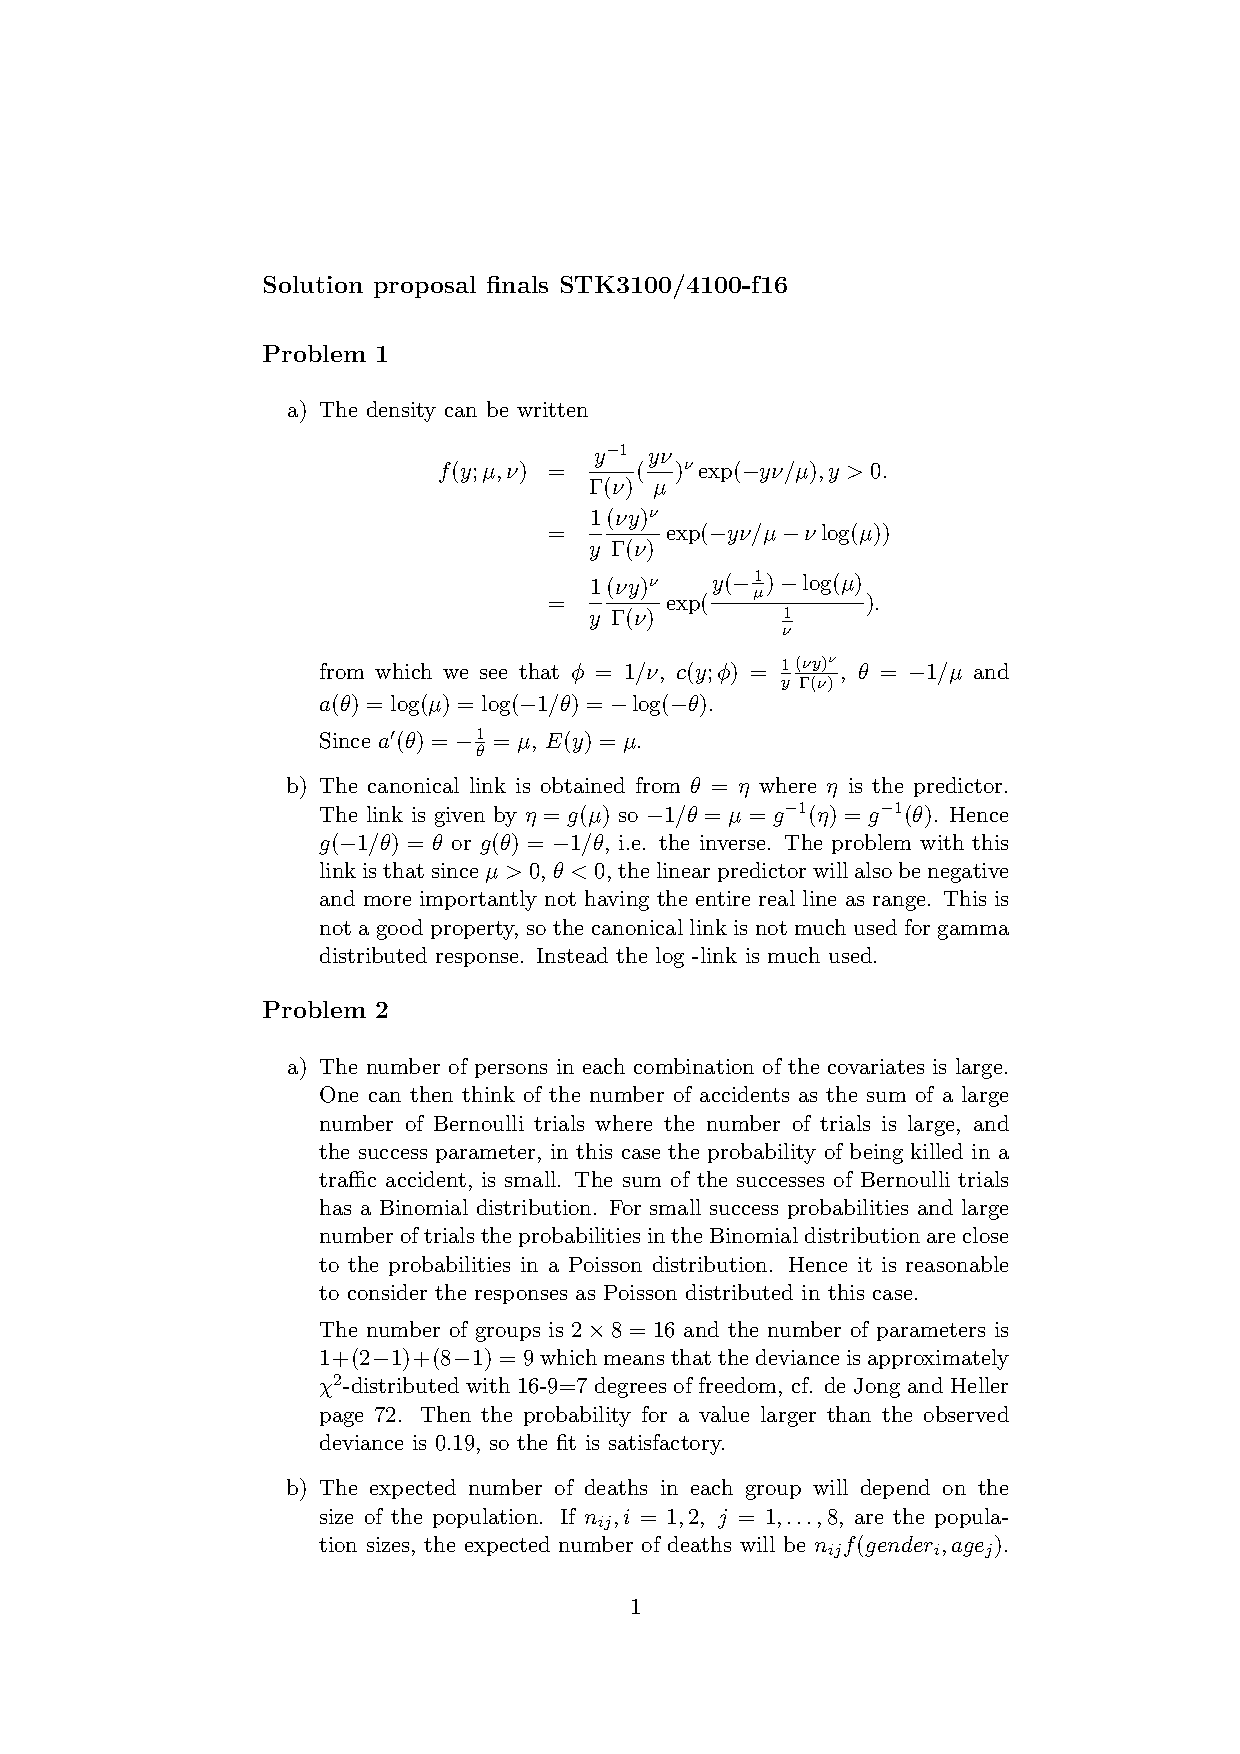
\includepdf[pages = {1, 2, 3}]{exam-exercises/exam-2016-solution.pdf}
\includepdf[pages = {2, 3, 4}]{exam-exercises/exam-2017-solution.pdf}
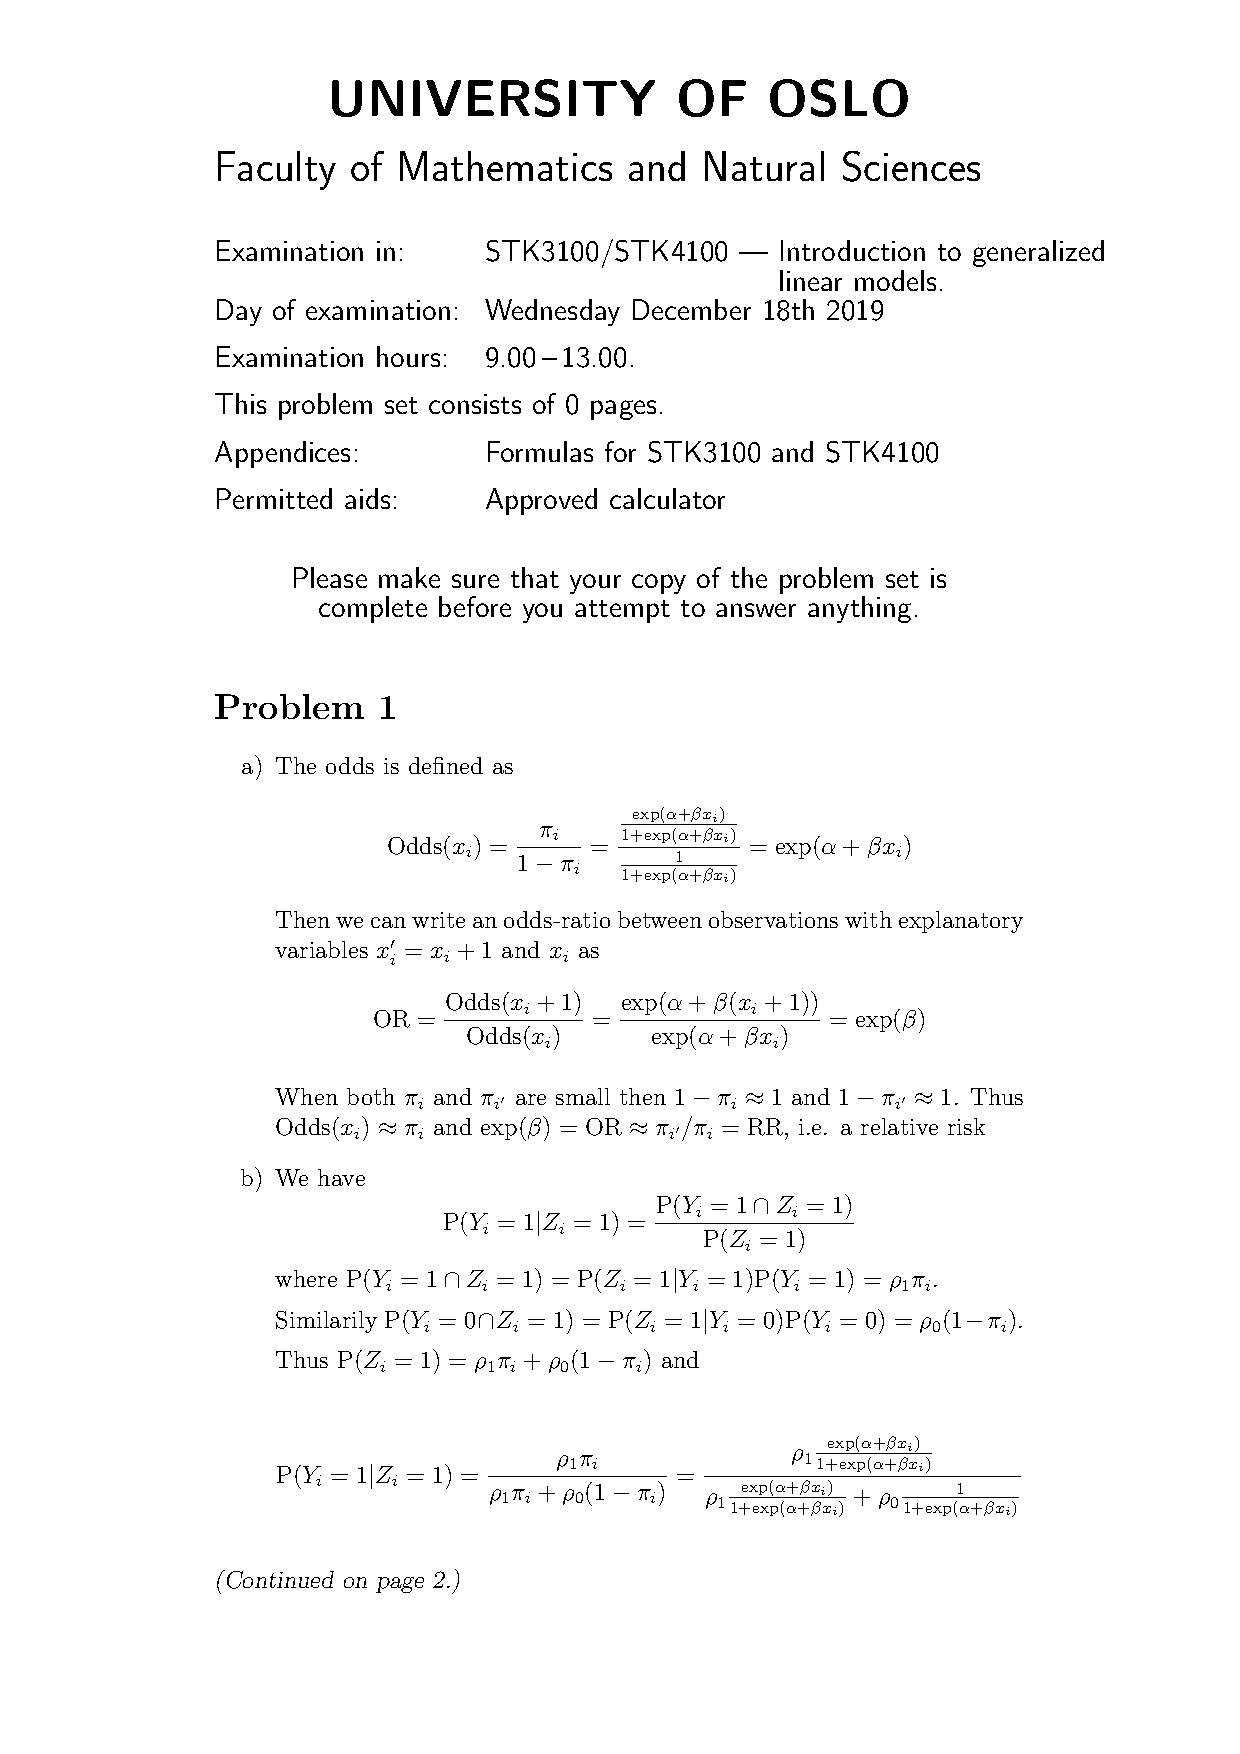
\includepdf[pages = {1, 2, 3}]{exam-exercises/exam-2019-solution.pdf}

\printbibliography
\end{document}
